% Apresentações em widescreen. Outros valores possíveis: 1610, 149, 54, 43 e 32.
% Por padrão, as apresentações são no formato 4:3 (sem o aspectratio).
\documentclass[aspectratio=169]{beamer}	 	

\renewcommand\textbullet{\ensuremath{\bullet}}

\usetheme{Pittsburgh}
\usecolortheme{default}
\usefonttheme[onlymath]{serif}			% para fontes matemáticas
% Enconte mais temas e cores em http://www.hartwork.org/beamer-theme-matrix/ 
% Veja também http://deic.uab.es/~iblanes/beamer_gallery/index.html
% Customizações de Cores: fg significa cor do texto e bg é cor do fundo
\setbeamercolor{normal text}{fg=black}
\setbeamercolor{alerted text}{fg=red}
\setbeamercolor{author}{fg=black}
\setbeamercolor{institute}{fg=black}
\setbeamercolor{date}{fg=black}
\setbeamercolor{frametitle}{fg=black}
\setbeamercolor{framesubtitle}{fg=brown}
\setbeamercolor{block title}{bg=black, fg=white}	%Cor do título
\setbeamercolor{block body}{bg=gray, fg=black}	%Cor do texto (bg= fundo; fg=texto)
\setbeamercolor{section in toc}{fg=black}
\setbeamercolor{section number projected}{bg=white,fg=black}
\setbeamercolor{titlelike}{fg=black}
% ---
% PACOTES
% ---
\usepackage[alf]{abntex2cite}	% Citações padrão ABNT
\usepackage[brazil]{babel}		% Idioma do documento
\usepackage{color}				% Controle das cores
\usepackage[T1]{fontenc}		% Selecao de codigos de fonte.
\usepackage{graphicx}			% Inclusão de gráficos
\usepackage[utf8]{inputenc}		% Codificacao do documento (conversão automática dos acentos)
\usepackage{txfonts}			% Fontes virtuais
\usepackage{bmpsize}
\usepackage[absolute,overlay]{textpos}
% ---

% --- Informações do documento ---
\title{Sistemas de Detecção e Prevenção de Intrusão - IDS/IPS}
\author{Glenon Mateus Barbosa Araújo}
%\institute{Universidade Federal do Pará \par Centro de Tecnologia da Informação e Comunicação}
\date{\today}
% ---

% ----------------- INÍCIO DO DOCUMENTO --------------------------------------
\begin{document}
\usebackgroundtemplate{
\includegraphics[width=1.5cm,height=\paperheight]{imagens/imagem.png}}
% ----------------- NOVO SLIDE --------------------------------
\begin{frame}
\begin{minipage}{\linewidth}
  \centering
  \begin{tabular}{cc}
    \begin{tabular}{c}
      \textbf{Universidade Federal do Pará} \\ 
      \textbf{Centro de Tecnologia da Informação e Comunicação}
    \end{tabular}
    &
    \begin{tabular}{c}
     
\includegraphics[width=4cm]{imagens/ctic-logo.png}
    \end{tabular}
  \end{tabular}
\end{minipage}
\titlepage
\end{frame}
% ----------------- NOVO SLIDE --------------------------------
\begin{frame}{Sumário}
  \tableofcontents
\end{frame}
% ----------------- NOVO SLIDE --------------------------------
\section{IDS/IPS}
\subsection{Definição}
\subsection{Tipos}
\begin{frame}{IDS/IPS}
  \framesubtitle{Definição}
  \begin{itemize}
	\item O que é Sistema de Detecção e Prevenção de Intrusão (IDS/IPS)?
	\begin{itemize}
		\item mecanismo capaz de identificar ou detectar a presença de atividades intrusivas
		\item processos utilizados na descoberta de utilizações não autorizadas de dispositivos de rede ou de computadores
		\item tem por objetivo impedir possíveis ataques
		\item trabalha maneira reativa e informativa
		\item diminui o risco de comprometimento de um ambiente 
	\end{itemize}
  \end{itemize}
\end{frame}

\begin{frame}{IDS/IPS}
	\framesubtitle{Tipos}
	\begin{itemize}
		\item \textit{Network Based}
			\begin{itemize}
				\item monitora o tráfego da rede
				\item analisa a rede e a atividade dos protocolos para identificar atividades suspeitas 			
			\end{itemize}				
		\item \textit{Host Based}
			\begin{itemize}
				\item monitora características do dispositivo e os eventos que acontecem no \textit{host}
				\item tráfego da rede para o dispositivo, os processos em execução, os \textit{logs} do sistema e o acesso e alteração em arquios e aplicações
			\end{itemize}
	\end{itemize}
\end{frame}

\begin{frame}{IDS/IPS}
	\framesubtitle{Tipos}
	\begin{itemize}
		\item Conhecimento
			\begin{itemize}
				\item banco de dados (assinaturas) de perfis de vulnerabilidades de sistemas já conhecidos, para identificar tentativas de intrusão ativas
				\item política de atualização continua das assinaturas
			\end{itemize}
		\item Comportamento
			\begin{itemize}
				\item analisa o comportamento do tráfego seguindo uma linha de base ou padrão de atividade normal do sistema
			\end{itemize}
	\end{itemize}		
\end{frame}

\begin{frame}{IDS/IPS}
	\framesubtitle{Tipos}
	\begin{itemize}
		\item Ativo
			\begin{itemize}
				\item bloqueia ataques e atividades suspeitas, sem qualquer intervenção humana
				\item importante uma parametrização adequada a fim de minimizar falsos positivos, bloqueando conexões legítimas
			\end{itemize}
		\item Passivo
			\begin{itemize}
				\item monitora o tráfego, identificando potenciais ataques, gerando alertas
				\item não interfere na comunicação
			\end{itemize}
	\end{itemize}
\end{frame}
% ----------------- NOVO SLIDE --------------------------------
\section{Fases de Implantação}
\subsection{Levantamento}
\subsection{Preparação do Ambiente}
\subsection{Testes}
\subsection{Avaliação}
\subsection{Conclusão}

\begin{frame}{Fases de Implantação}
  \framesubtitle{Levantamento}
  \begin{itemize}
  	\item Definir quais as ferramentas mais conhecidas de IDS/IPS
  		\begin{itemize}
  			\item Suricata
  			\item Snort
  		\end{itemize}
  	\item Identificar diferença entre elas
  		\begin{itemize}
  			\item \textit{multithread}
  		\end{itemize}
  \end{itemize}
\end{frame}

\begin{frame}{Fases de Implantação}
	\framesubtitle{Levantamento}
	\begin{textblock*}{5cm}(0cm,2cm) % {block width} (coords)		
		\centering Snort
		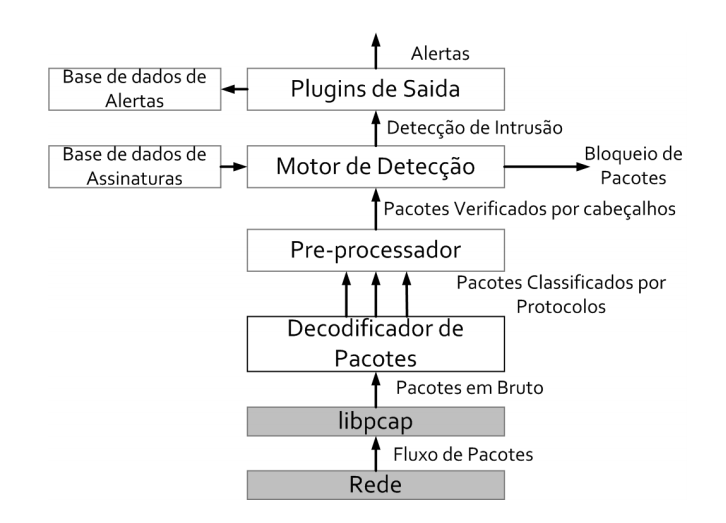
\includegraphics[width=8cm]{imagens/snort-arquitetura.png}
    \end{textblock*}
    \begin{textblock*}{5cm}(8cm,2cm) % {block width} (coords)
    	\centering Suricata
    	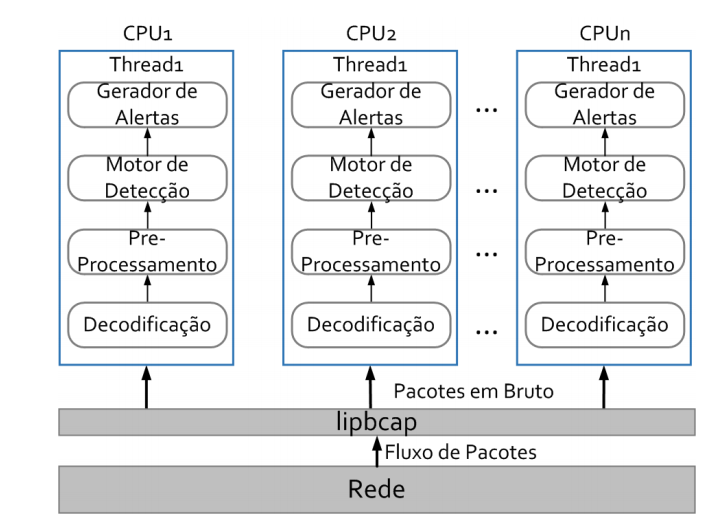
\includegraphics[width=8cm]{imagens/suricata-arquitetura.png}
    \end{textblock*}
\end{frame}

\begin{frame}{Fases de Implantação}
  \framesubtitle{Preparação do Ambiente}
  \begin{itemize}
  	\item Escolher uma rede com um tráfego considerado - ILC
  	\item \textit{Port mirroring} dessa rede para nosso servidor de teste
  	\item Instalação e configuração das VMs com as mesmas configurações (memória, processamento)
  	\item Problema com a formatação dos arquivos de logs do Snort (unified2 - json) - idstools-u2json
  \end{itemize}
\end{frame}

\begin{frame}{Fases de Implantação}
  \framesubtitle{Testes}
  \begin{itemize}
  	\item Escolha da base de assinaturas
 		\begin{itemize}
 			\item p2p
 			\item \textit{botnet}
 			\item DDOS
 			\item \textit{worms}
 			\item \textit{exploit}
 			\item \textit{scan}
 		\end{itemize}
 	\item Ferramentas para simulação de ataques
 		\begin{itemize}
 			\item Pytbull
 			\item Kali Linux
 		\end{itemize}
  \end{itemize}
\end{frame}

\begin{frame}{Fases de Implantação}
  \framesubtitle{Avaliação e Conclusão}
  \begin{itemize}
  	\item Análise do comportamento de cada IDS/IPS
  		\begin{itemize}
  			\item falsos positivos/negativos
  			\item quantidade de recurso usado num determinado período
  			\item quantidade de log gerado
  		\end{itemize}
  \end{itemize}
\end{frame}
\end{document}
